\documentclass[tikz,border=8pt]{standalone}

\usepackage[T1]{fontenc}
\usepackage{lmodern}
\usetikzlibrary{arrows.meta,backgrounds,fit,positioning}

\definecolor{inputblue}{HTML}{DCEBFA}
\definecolor{coregold}{HTML}{FFF0C2}
\definecolor{canopygreen}{HTML}{DDF2E3}
\definecolor{outputviolet}{HTML}{EADFF5}
\definecolor{linecolor}{HTML}{455A64}
\definecolor{labelcolor}{HTML}{263238}

\begin{document}
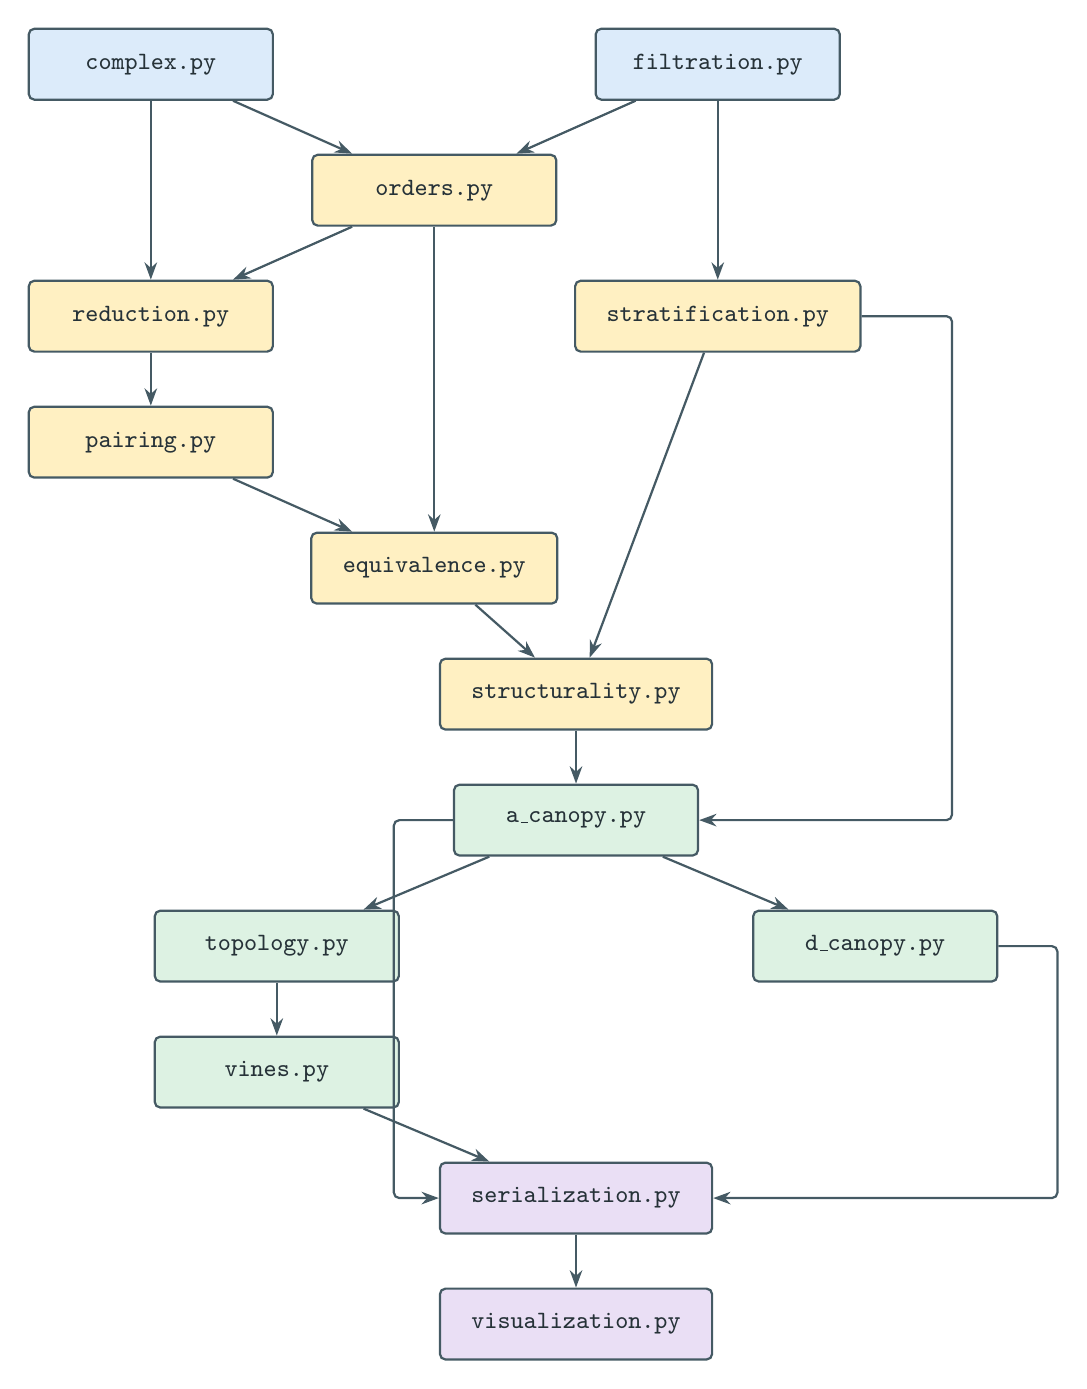
\begin{tikzpicture}[
  font=\sffamily,
  module/.style={
    draw=linecolor,
    line width=0.8pt,
    rounded corners=2pt,
    minimum width=31mm,
    minimum height=9mm,
    inner xsep=4mm,
    fill=white,
    text=labelcolor,
    font=\sffamily\small\ttfamily,
    align=center
  },
  input/.style={module,fill=inputblue},
  core/.style={module,fill=coregold},
  canopy/.style={module,fill=canopygreen},
  output/.style={module,fill=outputviolet},
  dependency/.style={
    -{Stealth[length=2.2mm,width=1.6mm]},
    draw=linecolor,
    line width=0.8pt,
    rounded corners=2pt
  }
]

% Input and algebraic core
\node[input]  (C) at (-3.6, 0.0) {complex.py};
\node[input]  (F) at ( 3.6, 0.0) {filtration.py};
\node[core]   (O) at ( 0.0,-1.6) {orders.py};
\node[core]   (R) at (-3.6,-3.2) {reduction.py};
\node[core]   (S) at ( 3.6,-3.2) {stratification.py};
\node[core]   (P) at (-3.6,-4.8) {pairing.py};
\node[core]   (E) at ( 0.0,-6.4) {equivalence.py};
\node[core]   (H) at ( 1.8,-8.0) {structurality.py};

% Canopy construction and topology
\node[canopy] (A) at ( 1.8,-9.6) {a\_canopy.py};
\node[canopy] (T) at (-2.0,-11.2) {topology.py};
\node[canopy] (D) at ( 5.6,-11.2) {d\_canopy.py};
\node[canopy] (V) at (-2.0,-12.8) {vines.py};

% Output layer
\node[output] (J) at ( 1.8,-14.4) {serialization.py};
\node[output] (Z) at ( 1.8,-16.0) {visualization.py};

% Dependencies
\draw[dependency] (C) -- (O);
\draw[dependency] (C) -- (R);
\draw[dependency] (F) -- (O);
\draw[dependency] (O) -- (R);
\draw[dependency] (R) -- (P);

\draw[dependency] (F) -- (S);
\draw[dependency] (O) -- (E);
\draw[dependency] (P) -- (E);
\draw[dependency] (E) -- (H);
\draw[dependency] (S) -- (H);

\draw[dependency] (H) -- (A);
\draw[dependency] (S.east) -- ++(1.15,0) |- (A.east);
\draw[dependency] (A) -- (T);
\draw[dependency] (A) -- (D);
\draw[dependency] (T) -- (V);

\draw[dependency] (A.west) -- ++(-0.75,0) |- (J.west);
\draw[dependency] (D.east) -- ++(0.75,0) |- (J.east);
\draw[dependency] (V) -- (J);
\draw[dependency] (J) -- (Z);

\end{tikzpicture}
\end{document}